\section{Eigenvalue method}
\label{eigenmethod:section}

\LAtt{3.4, 3.7}

\LO{
\item Use the eigenvalue method to find straight-line solutions to constant-coefficient first order systems of ODE,
\item Find general solutions to systems with real and distinct eigenvalues, and
\item Solve initial value problems from all of these cases once the general solution has been found. 
}

In this section we will learn how to solve linear homogeneous constant
coefficient systems of ODEs by the eigenvalue method.
Suppose we have such a system
\begin{equation*}
{\vec{x}}' = P\vec{x} ,
\end{equation*}
where
$P$ is a
constant square matrix.
We wish to
adapt the method for the single
constant coefficient equation by trying the function $e^{\lambda t}$.
However, $\vec{x}$ is a vector.  So we try $\vec{x} = \vec{v} e^{\lambda t}$, where
$\vec{v}$ is an arbitrary constant vector.  We plug this $\vec{x}$ into the equation to get
\begin{equation*}
\underbrace{\lambda \vec{v} e^{\lambda t}}_{{\vec{x}}'} =
\underbrace{P\vec{v} e^{\lambda t}}_{P\vec{x}} .
\end{equation*}
We divide by $e^{\lambda t}$ and notice that we are looking for a scalar $\lambda$
and a vector $\vec{v}$ that satisfy the equation
\begin{equation*}
\lambda \vec{v} = P\vec{v} .
\end{equation*}

This means that we are looking for an eigenvalue $\lambda$ with corresponding eigenvector $\vec{v}$ for the matrix $P$. When we can find these, we will get solutions to the original system of differential equations of the form \[ \vec{x}(t) = \vec{v}e^{\lambda t}. \] We get the easiest route to solutions when the matrix $P$ has all real eigenvalues and the eigenvalues are all distinct, and can extend to deal with the complications that arise from complex and repeated eigenvalues.  

Another way to view these types of solutions are as ``straight-line solutions.'' A system of differential equations of the form 
\begin{equation*}
{\vec{x}}' = P\vec{x} ,
\end{equation*}
is an autonomous system of differential equations, because there is no explicit dependence on $t$ on the right-hand side. When we solved autonomous equations in \sectionref{auteq:section}, we started by looking for equilibrium solutions and built up from there. In this particular case, we are looking for vectors $\vec{x}$ so that $P\vec{x} = 0$. As long as $P$ is invertible, the only vector that satisfies this is $\vec{x} = 0$. So, that's not super interesting, and doesn't really tell us too much about the solution to the problem.

\begin{mywrapfig}{3.25in}
\capstart
\myincludegraphics{width=2in}{width=3in}{eigen-straight-line}
\caption{Position vector and possible direction vectors for straight line solutions.\label{posdir:source-eigfig}}
\end{mywrapfig}

The next more involved type of solution we could look for is a straight-line solution. The idea is that this solution will either move directly (in a straight-line) towards or away from the origin. In the first order autonomous equation case, all of our solutions did this; they either moved towards or away from these equilibrium solutions. This may not be the case for systems, but we can try to find them. If a solution is going to move directly towards or away from the origin, then the direction of change for the solution must be parallel to the position vector. In \figurevref{posdir:source-eigfig}, the vectors that point in the same or opposite direction of $\vec{x}$ will give rise to a straight-line solution, but vectors that do not point in this direction will give solutions that do not follow a straight-line through the origin. 

This criterion means that we need to have 
\begin{equation*}
\vec{x}' = \lambda \vec{x}
\end{equation*}
for some constant $\lambda$. If this is the case, then we have 
\begin{equation*}
P\vec{x} = \lambda \vec{x}
\end{equation*}
and this is the equation for eigenvalues and eigenvectors of $P$. We are back to the same type of solution that we found previously.

\subsection{The eigenvalue method with distinct real eigenvalues}

OK\@.  We have the system of equations
\begin{equation*}
{\vec{x}}' = P\vec{x} .
\end{equation*}
We find the eigenvalues $\lambda_1$, $\lambda_2$, \ldots, $\lambda_n$
of the matrix $P$, and corresponding eigenvectors
$\vec{v}_1$, $\vec{v}_2$, \ldots, $\vec{v}_n$.
Now we notice that the functions
$\vec{v}_1 e^{\lambda_1 t}$, 
$\vec{v}_2 e^{\lambda_2 t}$, \ldots,
$\vec{v}_n e^{\lambda_n t}$ are solutions of the homogeneous system of equations and hence
$
\vec{x} = c_1 \vec{v}_1 e^{\lambda_1 t} +
c_2 \vec{v}_2 e^{\lambda_2 t} + \cdots +
c_n \vec{v}_n e^{\lambda_n t}
$
is a solution by superposition.

\begin{theorem1}{}
Take ${\vec{x}}' = P\vec{x}$.  If $P$ is an $n \times n$ constant matrix
that
has $n$ distinct real eigenvalues $\lambda_1$, $\lambda_2$, \ldots, $\lambda_n$,
then there exist $n$ linearly independent corresponding eigenvectors
$\vec{v}_1$, $\vec{v}_2$, \ldots, $\vec{v}_n$, and the general solution to
${\vec{x}}' = P\vec{x}$
can be written as
\begin{equation*}
%\mybxbg{~~
\vec{x} = c_1 \vec{v}_1 e^{\lambda_1 t} +
c_2 \vec{v}_2 e^{\lambda_2 t} + \cdots +
c_n \vec{v}_n e^{\lambda_n t} .
%~~}
\end{equation*}
\end{theorem1}

The corresponding fundamental matrix solution is
\begin{equation*}
X(t) = \bigl[\, \vec{v}_1 e^{\lambda_1 t} \quad \vec{v}_2 e^{\lambda_2 t}
\quad \cdots \quad \vec{v}_n e^{\lambda_n t} \,\bigr].
\end{equation*}
That is, $X(t)$
is the matrix whose $j^{\text{th}}$ column is 
$\vec{v}_j e^{\lambda_j t}$.

\begin{example}
Consider the system
\begin{equation*}
{\vec{x}}'
=
\begin{bmatrix}
2 & 1 & 1 \\
1 & 2 & 0 \\
0 & 0 & 2
\end{bmatrix}
\vec{x} .
\end{equation*}
Find the general solution.
\end{example}

\begin{exampleSol}
Earlier, we found the eigenvalues are $1,2,3$.  We found the eigenvector
$\left[ \begin{smallmatrix} 1 \\ 1 \\ 0 \end{smallmatrix} \right]$
for the eigenvalue 3.  Similarly
we find the eigenvector 
$\left[ \begin{smallmatrix} 1 \\ -1 \\ 0 \end{smallmatrix} \right]$
for the eigenvalue 1, and 
$\left[ \begin{smallmatrix} 0 \\ 1 \\ -1 \end{smallmatrix} \right]$
for the eigenvalue 2 (exercise: check).
Hence our general solution is
\begin{equation*}
\vec{x} =
c_1
\begin{bmatrix}
1 \\ -1 \\ 0
\end{bmatrix}
e^t
+
c_2
\begin{bmatrix}
0 \\ 1 \\ -1
\end{bmatrix}
e^{2t}
+
c_3
\begin{bmatrix}
1 \\ 1 \\ 0
\end{bmatrix}
e^{3t} 
=
\begin{bmatrix}
c_1 e^t+c_3 e^{3t} \\ -c_1 e^t + c_2 e^{2t} + c_3 e^{3t} \\ - c_2 e^{2t}
\end{bmatrix} .
\end{equation*}
In terms of a fundamental matrix solution,
\begin{equation*}
\vec{x} = X(t)\, \vec{c}
=
\begin{bmatrix}
e^t & 0 & e^{3t} \\
-e^t & e^{2t} & e^{3t} \\
0 & -e^{2t} & 0
\end{bmatrix}
\begin{bmatrix}
c_1 \\ c_2 \\ c_3
\end{bmatrix} .
\end{equation*}
\end{exampleSol}

\begin{exercise}
Check that this $\vec{x}$ really solves the system.
\end{exercise}

Overall, the process for finding the solution for real and distinct eigenvalues is to first find the eigenvalues and eigenvectors of the matrix $P$. Once we have these, we get $n$ linearly independent solutions of the form $\vec{x}_i(t) = \vec{v}_ie^{\lambda_i t}$, so that the general solution is of the form
\[ \vec{x}(t) = c_1\vec{v}_1e^{\lambda_1 t} + c_2\vec{v}_2e^{\lambda_2 t} + \cdots + c_n\vec{v}_ne^{\lambda_n t}. \] Then, if we need to solve for an initial condition, we figure out the coefficients $c_1$, $c_2$, ..., $c_n$ to satisfy this condition.

Note: If we write a single homogeneous linear constant coefficient $n^{\text{th}}$
order equation as a first order system (as we did in \sectionref{sec:introtosys}),
then the eigenvalue equation
\begin{equation*}
\det(P - \lambda I) = 0
\end{equation*}
is essentially the same as the characteristic equation we got in
\sectionref{solinear:section} and
\sectionref{sec:hol}. See the exercises for details about this.

\begin{example}
Solve the initial value problem
\begin{equation*}
\vec{x}' = \begin{bmatrix} 0 & 4 \\ -3 & -7 \end{bmatrix}\vec{x} \qquad \vec{x}(0) = \begin{bmatrix} 1 \\ 1 \end{bmatrix}.
\end{equation*}
\end{example}

\begin{exampleSol}
Since we are in the case of a constant-coefficient linear system, we start by looking for the eigenvalues and eigenvectors of the coefficient matrix $P$. To do this, we compute
\begin{equation*}
\det(P - \lambda I) = (0-\lambda)(-7-\lambda) - (4)(-3) = \lambda^2 + 7\lambda + 12.
\end{equation*}
This polynomial factors as $(\lambda + 3)(\lambda + 4)$, and so the two eigenvalues are $\lambda_1 = -3$ and $\lambda_2 = -4$. 

Next, we need to find the corresponding eigenvectors. For $\lambda = -3$, we get the matrix equation
\begin{equation*}
(P + 3I)\vec{v} = \begin{bmatrix} 3 & 4 \\ -3 & -4 \end{bmatrix} \vec{v} = \vec{0}. 
\end{equation*}
The two equations that you get here are redundant, which is $3v_1 + 4v_2 = 0$. One way to satisfy this is $v_1 = 4$, $v_2 = -3$, so that the eigenvector is $\left[\begin{smallmatrix} 4 \\ -3 \end{smallmatrix} \right]$. 

For $\lambda = -4$, the matrix becomes
\begin{equation*}
(P + 4I)\vec{v} = \begin{bmatrix} 4 & 4 \\ -3 & -3 \end{bmatrix}\vec{v} = 0
\end{equation*}
so the eigenvector here is $\left[ \begin{smallmatrix} 1 \\ -1 \end{smallmatrix} \right]$. Therefore, the general solution to this differential equation, by superposition, is
\begin{equation*}
\vec{x}(t) = c_1 \begin{bmatrix} 4 \\ -3 \end{bmatrix}e^{-3t} + c_2 \begin{bmatrix} 1 \\ -1 \end{bmatrix}e^{-4t}.
\end{equation*}

Finally, we have to solve the initial value problem using the initial conditions. If we plug in $t=0$, we get the equation
\begin{equation*}
\vec{x}(0) = c_1 \begin{bmatrix} 4 \\ -3 \end{bmatrix} + c_2 \begin{bmatrix} 1 \\ -1 \end{bmatrix} = \begin{bmatrix} 1 \\ 1 \end{bmatrix}.
\end{equation*}
This results in needing to solve the system of equations
\begin{equation*}
4c_1 + c_2 = 1 \qquad -3c_1 - c_2 = 1.
\end{equation*}
These can be solved in any way, including row reduction. We will start by adding the two equations together, which gives $c_1 = 2$, and then the first equation implies that $c_2 = -7$. Therefore, the solution to the initial value problem is
\begin{equation*}
\vec{x}(t) = 2 \begin{bmatrix} 4 \\ -3 \end{bmatrix}e^{-3t}  - 7 \begin{bmatrix} 1 \\ -1 \end{bmatrix}e^{-4t} = \begin{bmatrix} 8e^{-3t} - 7e^{-4t} \\ -6e^{-3t} + 7e^{-4t} \end{bmatrix}.
\end{equation*}
\end{exampleSol}

\subsection{Phase Portraits}

Now that we have these solutions, we want to get an idea for what they look like in the plane. We spent a lot of time in first order equations looking at direction fields, as well as phase lines for autonomous equations. We want to develope the same type of intuition for two-component systems in the plane, because much intuition can be obtained by studying this simple case.
Suppose we use coordinates $(x,y)$ for the plane as usual,
and suppose
$P = \left[ \begin{smallmatrix} a & b \\ c & d \end{smallmatrix} \right]$ 
is a $2 \times 2$ matrix.  Consider the system
\begin{equation} \label{pln:eq}
\begin{bmatrix} x \\ y \end{bmatrix} ' =
P \begin{bmatrix} x \\ y \end{bmatrix} 
\qquad 
\text{or}
\qquad
\begin{bmatrix} x \\ y \end{bmatrix} ' =
\begin{bmatrix} a & b \\ c & d \end{bmatrix} 
\begin{bmatrix} x \\ y \end{bmatrix} 
.
\end{equation}
The system is autonomous (compare this section
to \sectionref{auteq:section})
and so we can draw a vector field (see the end of
\sectionref{sec:introtosys}).
We will be able to visually tell what the vector field looks like and
how the solutions behave, once we find 
the eigenvalues and eigenvectors of the matrix $P$. The goal is to be able to sketch what the different trajectories of the solutions look like for a variety of initial conditions, as well as classify the general type of picture that results depending on the matrix $P$. 
% For this section, we assume that $P$ has two eigenvalues and two corresponding eigenvectors.

\medskip

\emph{Case 1.}  Suppose that the eigenvalues of $P$ are real and positive.
We find two corresponding eigenvectors and plot them in the plane.  For
example, take the
matrix $\left[ \begin{smallmatrix} 1 & 1 \\ 0 & 2 \end{smallmatrix}
\right]$.
The eigenvalues are 1 and 2 and corresponding eigenvectors are
$\left[ \begin{smallmatrix} 1 \\ 0 \end{smallmatrix} \right]$ and
$\left[ \begin{smallmatrix} 1 \\ 1 \end{smallmatrix} \right]$.  See
\figurevref{pln:source-eigfig}.

\begin{mywrapfig}{3.25in}
\capstart
\diffyincludegraphics{width=3in}{width=4.5in}{pln-source-eig}
\caption{Eigenvectors of $P$.\label{pln:source-eigfig}}
\end{mywrapfig}

Suppose the point $(x,y)$ is on the line determined by an eigenvector
$\vec{v}$ for an eigenvalue $\lambda$.
That is,
$\left[ \begin{smallmatrix} x \\ y \end{smallmatrix} \right] = \alpha \vec{v}$
for some scalar $\alpha$.
Then 
\begin{equation*}
\begin{bmatrix} x \\ y \end{bmatrix} '
=
P \begin{bmatrix} x \\ y \end{bmatrix}
=
P ( \alpha \vec{v} ) =  \alpha ( P \vec{v} )
= \alpha \lambda \vec{v} .
\end{equation*}
The derivative is a multiple of $\vec{v}$ and hence points along the
line determined by $\vec{v}$.  As $\lambda > 0$, the derivative points in the
direction of $\vec{v}$ when $\alpha$ is positive and in the opposite direction
when $\alpha$ is negative.  Let us draw the lines determined by
the eigenvectors, and let us draw
arrows on the lines to indicate the directions.
See \figurevref{pln:source-eig-arrfig}.

We fill in the rest of the arrows for the vector field
and we also draw a few solutions.  See
\figurevref{pln:source-fullfig}.
The picture looks like a source
with arrows coming out from the origin.
Hence we call this type of picture a
\emph{\myindex{source}} or sometimes an \emph{\myindex{unstable node}}. Notice the two eigenvectors are drawn on the entire vector field figure with arrows, and the straight-line solutions follow them.  

\begin{myfig}
\parbox[t]{3.0in}{
 \capstart
 \diffyincludegraphics{width=3in}{width=4.5in}{pln-source-eig-arr}
 \caption{Eigenvectors of $P$ with directions.\label{pln:source-eig-arrfig}}
}
\quad
\parbox[t]{3.0in}{
 \capstart
 \diffyincludegraphics{width=3in}{width=4.5in}{pln-source-full}
 \caption{Example source vector field with eigenvectors and
 solutions.\label{pln:source-fullfig}}
}
\end{myfig}

\medskip

\emph{Case 2.} Suppose both eigenvalues are negative.  For example, take
the
negation of the matrix in case 1,
$\left[ \begin{smallmatrix} -1 & -1 \\ 0 & -2 \end{smallmatrix} \right]$.
The eigenvalues are $-1$ and $-2$ and corresponding eigenvectors are
the same,
$\left[ \begin{smallmatrix} 1 \\ 0 \end{smallmatrix} \right]$ and
$\left[ \begin{smallmatrix} 1 \\ 1 \end{smallmatrix} \right]$.  The
calculation and the picture are almost the same.  The only difference is that
the eigenvalues are negative and hence all arrows are reversed.  We get the
picture in \figurevref{pln:sink-fullfig}.  We call this kind of picture a
\emph{\myindex{sink}} or a \emph{\myindex{asymptotically stable node}}.

\begin{myfig}
\parbox[t]{3.0in}{
 \capstart
 \diffyincludegraphics{width=3in}{width=4.5in}{pln-sink-full}
 \caption{Example sink vector field with eigenvectors and
 solutions.\label{pln:sink-fullfig}}
}
\quad
\parbox[t]{3.0in}{
 \capstart
 \diffyincludegraphics{width=3in}{width=4.5in}{pln-saddle-full}
 \caption{Example saddle vector field with eigenvectors and
 solutions.\label{pln:saddle-fullfig}}
}
\end{myfig}

\medskip

\emph{Case 3.} Suppose one eigenvalue is positive and one is negative.
For example the matrix
$\left[ \begin{smallmatrix} 1 & 1 \\ 0 & -2 \end{smallmatrix} \right]$.
The eigenvalues are 1 and $-2$ and corresponding eigenvectors are
$\left[ \begin{smallmatrix} 1 \\ 0 \end{smallmatrix} \right]$ and
$\left[ \begin{smallmatrix} 1 \\ -3 \end{smallmatrix} \right]$.  We reverse
the arrows on one line (corresponding to the negative eigenvalue) and we
obtain the picture in \figurevref{pln:saddle-fullfig}.  We call this picture a
\emph{\myindex{saddle point}}.


\subsection{Exercises}

\begin{exercise}
\leavevmode
\begin{tasks}
\task
Find the general solution of $x_1' = 2 x_1$, $x_2' = 3 x_2$ using the
eigenvalue method (first write the system in the form
${\vec{x}}' = A \vec{x}$).
\task
Solve the system by solving each equation
separately and verify you get the same general solution.
\end{tasks}
\end{exercise}
\comboSol{%
}
{%
$C_1\left[\begin{smallmatrix} 1 \\ 0 \end{smallmatrix}\right]e^{2t} + C_2\left[\begin{smallmatrix} 0 \\ 1  \end{smallmatrix}\right]e^{3t}$
}

\begin{exercise}
Find the general solution of $x_1' = 3 x_1 + x_2$,
$x_2' = 2 x_1 + 4 x_2$ using the eigenvalue method and sketch the phase portrait for this system of differential equations.
\end{exercise}
\comboSol{%
}
{%
$C_1 \left[\begin{smallmatrix} 1 \\ -1 \end{smallmatrix}\right]e^{2t} + C_2\left[\begin{smallmatrix} 1 \\ 2 \end{smallmatrix}\right]e^{-t}$ \hfill
\raisebox{-0.5\height}{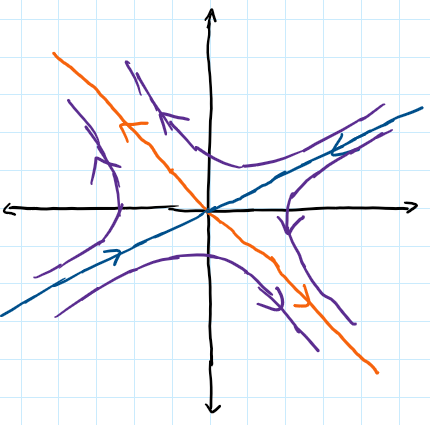
\includegraphics[height=1.5in]{Images/phaseportrait_3_1_2_4_sketch.png}} \hfill \hfill
}

\begin{exercise}\ansMark%
Solve $x_1' = x_2$, $x_2' = x_1$ using the eigenvalue method and sketch the phase portrait for this system of differential equations.
\end{exercise}
\exsol{%
$\vec{x} = C_1 \left[ \begin{smallmatrix}
1 \\ 1
\end{smallmatrix}\right] e^{t}
+
C_2 \left[ \begin{smallmatrix}
1 \\ -1
\end{smallmatrix}\right] e^{-t}$ \hfill
\raisebox{-0.5\height}{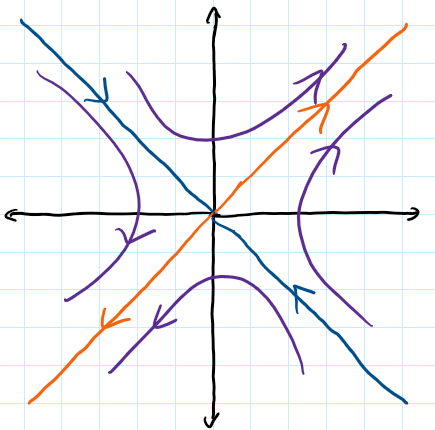
\includegraphics[height=1.5in]{Images/phaseportrait_0_1_1_0_sketch.png}} \hfill\hfill
}


\begin{exercise}
Amino acid dating can be used by forensic scientists to determine the time of death in situations where other techniques might not work. These amino acids are sneaky, and they exist in a left-handed form (L) and a right-handed form (D), which are called {\it enantiomers}. While you’re alive, your body keeps all your amino acids in the L form. Once you die, your body no longer regulates your amino acids, and every so often they flip a coin and decide whether to switch into the opposite form. This way, when someone finds your body in a dumpster, they can pull out your teeth and measure the {\it racemization ratio}, which is the ratio of D-enantiomers to L-enantiomers. %4.4

Denote by $D(t)$ and $L(t)$, respectively, the proportions of D- and L-enantiomers found in your teeth, where $t$ is measured in years after death. Since this is Math class, the proportions are governed by a system of differential equations, such as
\begin{equation}
\begin{bmatrix} L' \\ D' \end{bmatrix} = \begin{bmatrix} -.02& .02\\ .02 & -.02 \end{bmatrix}\begin{bmatrix} L\\ D \end{bmatrix}.\label{eq:AminoEqn}
\end{equation}
\begin{tasks}
\task Find the general solution to \eqref{eq:AminoEqn}.
\task Solve \eqref{eq:AminoEqn} with initial conditions $D(0) = 0$ and $L(0) = 1$, and express the solution in component form. Describe what happens to the quantities $D(t)$ and $L(t)$ in the long run.
\task Given the above initial conditions, if the racemization ratio in your teeth is currently 1:3, how long ago did you die?
\end{tasks}
\end{exercise}
\comboSol{%
}
{%
a)~ $\vec{x}(t) = C_1 \left[\begin{smallmatrix} -1 \\ 1 \end{smallmatrix}\right]e^{-t/25} + C_2\left[\begin{smallmatrix} 1 \\ 1 \end{smallmatrix}\right]$ \\ b)~ $L(t) = \frac{1}{2} + \frac{1}{2}e^{-t/25},\ D(t) = \frac{1}{2} - \frac{1}{2}e^{-t/25}$. Both go to $1/2$. \\ c)~ $t = 25\ln(2)\approx 17.33$ years
}

\begin{exercise}
\leavevmode
\begin{tasks}
\task
Compute eigenvalues and eigenvectors of
$A = \left[ \begin{smallmatrix}
9 & -2 & -6 \\
-8 & 3 & 6 \\
10 & -2 & -6
\end{smallmatrix} \right]$.
\task
Find the general solution of ${\vec{x}}' = A \vec{x}$.
\end{tasks}
\end{exercise}
\comboSol{%
}
{%
a)~ $\lambda_1 = 1$, $\vec{v}_1 = \left[\begin{smallmatrix} 1/2 \\ -1 \\ 1 \end{smallmatrix}\right]$. $\lambda_2 = 2$, $\vec{v}_2 = \left[\begin{smallmatrix} 2 \\ -2 \\ 3 \end{smallmatrix}\right]$. $\lambda_3 = 3$, $\vec{v}_3 = \left[\begin{smallmatrix} 3 \\ -3 \\ 4 \end{smallmatrix}\right]$ \\
b)~ $\vec{x}(t) = C_1\left[\begin{smallmatrix} 1/2 \\ -1 \\ 1 \end{smallmatrix}\right]e^t + C_2\left[\begin{smallmatrix} 2 \\ -2 \\ 3 \end{smallmatrix}\right]e^{2t} + C_3\left[\begin{smallmatrix} 3 \\ -3 \\ 4 \end{smallmatrix}\right]e^{3t}$
}

\begin{exercise}\ansMark%
\leavevmode
\begin{tasks}
\task
Compute eigenvalues and eigenvectors of
$A= \left[ \begin{smallmatrix}
1 & 0 & 3 \\
-1 & 0 & 1 \\
2 & 0 & 2
\end{smallmatrix}\right]$.
\task
Solve the system
$\vec{x}\,' = A \vec{x}$.
\end{tasks}
\end{exercise}
\exsol{%
a)
Eigenvalues: $4,0,-1$
\quad
Eigenvectors:
$\left[ \begin{smallmatrix}
1 \\ 0 \\ 1
\end{smallmatrix}\right]$,
$\left[ \begin{smallmatrix}
0 \\ 1 \\ 0
\end{smallmatrix}\right]$,
$\left[ \begin{smallmatrix}
3 \\ 5 \\ -2
\end{smallmatrix}\right]$
\\
b)
$\vec{x} = 
C_1
\left[ \begin{smallmatrix}
1 \\ 0 \\ 1
\end{smallmatrix}\right] e^{4t}
+
C_2
\left[ \begin{smallmatrix}
0 \\ 1 \\ 0
\end{smallmatrix}\right] +
C_3
\left[ \begin{smallmatrix}
3 \\ 5 \\ -2
\end{smallmatrix}\right] e^{-t}$
}

\begin{exercise}
Let $a,b,c,d,e,f$ be numbers.  Find the eigenvalues of
$\left[ \begin{smallmatrix}
a & b & c \\
0 & d & e \\
0 & 0 & f \\
\end{smallmatrix} \right]$.
\end{exercise}
\comboSol{%
}
{%
a, d, f
}

\begin{exercise}\ansMark%
Find the general solution of the system
\begin{equation*}
{\vec{x}}' = \begin{bmatrix} -7 & 1 \\ -12 & 0 \end{bmatrix} \vec{x}
\end{equation*}
and sketch the phase portrait for this system.
\end{exercise}
\exsol{%
$\displaystyle \vec{x}(t) = C_1 \left[\begin{smallmatrix} 1 \\ 3 \end{smallmatrix}\right]e^{-4t} + C_2 \left[\begin{smallmatrix} 1 \\ 4 \end{smallmatrix}\right] e^{-3t}$ \hfill
\raisebox{-0.5\height}{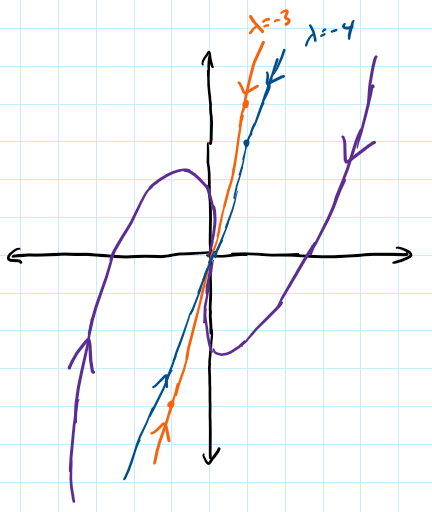
\includegraphics[height=1.5in]{Images/phaseportrait_n7_1_n12_0_sketch.png}}\hfill\hfill
}%

\begin{exercise}\ansMark%
Find the general solution of the system
\begin{equation*}
{\vec{x}}' = \begin{bmatrix} -13 & -12 \\ 9 & 8 \end{bmatrix} \vec{x}
\end{equation*}
and draw a sketch for the phase portrait.
\end{exercise}
\exsol{%
$\displaystyle \vec{x}(t) = C_1 \left[\begin{smallmatrix} -4 \\ 3 \end{smallmatrix}\right]e^{-4t} + C_2 \left[\begin{smallmatrix} 1 \\ -1 \end{smallmatrix}\right] e^{-t}$ \hfill
\raisebox{-0.5\height}{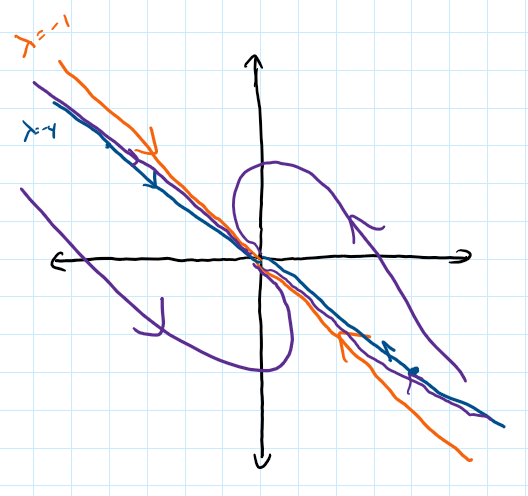
\includegraphics[height=1.5in]{Images/phaseportrait_n13_n12_9_8_sketch.png}}\hfill\hfill
}%

\begin{exercise}\ansMark%
Find the general solution of the system
\begin{equation*}
{\vec{x}}' = \begin{bmatrix} -2 & -6 & 0 \\ 4 & 8 & 0 \\ -4 & -7 & 3 \end{bmatrix} \vec{x}.
\end{equation*}
\end{exercise}
\exsol{%
$\displaystyle \vec{x}(t) = C_1 \left[\begin{smallmatrix} 0 \\ 0 \\ 1 \end{smallmatrix}\right]e^{3t} + C_2 \left[\begin{smallmatrix} -1 \\ 1 \\ -3 \end{smallmatrix}\right] e^{4t} + C_3 \left[\begin{smallmatrix} 3 \\ -2 \\ -2 \end{smallmatrix}\right] e^{2t}$
}%

\begin{exercise}\ansMark%
Find the general solution of the system
\begin{equation*}
{\vec{x}}' = \begin{bmatrix} -6 & 2 & 4 \\ -2 & -1 & 4 \\ -2 & 1 & 0 \end{bmatrix} \vec{x}.
\end{equation*}
\end{exercise}
\exsol{%
$\displaystyle \vec{x}(t) = C_1 \left[\begin{smallmatrix} 2 \\ 0 \\ 1 \end{smallmatrix}\right]e^{-4t} + C_2 \left[\begin{smallmatrix} 2 \\ 3 \\ 1 \end{smallmatrix}\right] e^{-t} + C_3 \left[\begin{smallmatrix} 1 \\ 2 \\ 0 \end{smallmatrix}\right] e^{-2t}$
}%

\begin{exercise}
Solve the initial value problem
\[ {\vec{x}}' = \begin{bmatrix} -3 & 0 \\ 3 & -4 \end{bmatrix} \vec{x} \qquad \vec{x}(0) = \begin{bmatrix} -1 \\ 2 \end{bmatrix}. \]
\end{exercise}
\comboSol{%
}
{%
$\vec{x}(t) = -\left[\begin{smallmatrix} 1 \\ 3 \end{smallmatrix}\right]e^{-3t} + 5\left[\begin{smallmatrix} 0 \\ 1 \end{smallmatrix}\right]e^{-4t}$
}

\begin{exercise}
Solve the initial value problem
\[ {\vec{x}}' = \begin{bmatrix} 1 & -3 \\ 2 & 6 \end{bmatrix} \vec{x} \qquad \vec{x}(0) = \begin{bmatrix} 1 \\ 1 \end{bmatrix}. \]
\end{exercise}
\comboSol{%
}
{%
$\vec{x}(t) = -5\left[\begin{smallmatrix} 1 \\ -1 \end{smallmatrix}\right]e^{4t} + 2\left[\begin{smallmatrix} 3 \\ -2 \end{smallmatrix}\right]e^{3t}$
}

\begin{exercise}
Solve the initial value problem
\[ {\vec{x}}' = \begin{bmatrix} 7 & 4 & 0 \\ -8 & -5 & 0 \\ 17 & 7 & -2 \end{bmatrix} \vec{x} \qquad \vec{x}(0) = \begin{bmatrix} -3 \\ 2 \\ 2 \end{bmatrix}. \]
\end{exercise}
\comboSol{%
}
{%
$\vec{x}(t) = \left[\begin{smallmatrix} 1 \\ -2 \\ 3 \end{smallmatrix}\right]e^{-t} + 7\left[\begin{smallmatrix} 0 \\ 0 \\ 1 \end{smallmatrix}\right]e^{-2t} - 4\left[\begin{smallmatrix} 1 \\ -1 \\ 2 \end{smallmatrix}\right]e^{3t}$
}


\setcounter{exercise}{100}












